% Shared preamble for the English summaries in this repository.
\documentclass[11pt,a4paper]{article}
\usepackage[margin=2.2cm]{geometry}
\usepackage[T1]{fontenc}
\usepackage[utf8]{inputenc}
\usepackage{lmodern}
\usepackage{amsmath,amssymb}
\usepackage{graphicx}
\usepackage{booktabs}
\usepackage{enumitem}
\usepackage[hidelinks]{hyperref}
\setlist{itemsep=2pt,topsep=4pt}
\setlength{\parindent}{0pt}
\setlength{\parskip}{5pt}
\graphicspath{{figures/}}
\newcommand{\summaryheader}[3]{%
  \begin{center}
    {\Large\bfseries #2}\\[3pt]
    {\large #1}\\[3pt]
    {\small Arshia Goshtasbi \textbullet{} MSc Electrical Engineering (Control), Iran University of Science and Technology \textbullet{} #3}
  \end{center}
  \vspace{2pt}\hrule\vspace{8pt}
  \noindent\textit{English summary of my original Persian report, which is kept as a PDF in this folder.}\par}

\begin{document}
\summaryheader{Optimal Control, Homework 8}{Dynamic Programming on a Grid}{Spring 1404 (2025)}

\section*{Problem}
The system is $x(k+1)=x(k)+u(k)$, with $0\le x\le 1.5$, $|u|\le 1$ and $x(0)=1.5$. The cost is $J=x(N)^2+\sum_{k=0}^{N-1}2u(k)^2$, minimised by backward dynamic programming on quantised state and input grids.

\section*{Method (\texttt{Q8.m})}
The terminal cost $J_N(x)=x^2$ is stored on the state grid. Going backwards, for every grid state I try every grid input that keeps $x(k+1)$ feasible, interpolate the cost-to-go, and keep the best input. A forward pass from $x_0$ then recovers the optimal trajectory.

\section*{Results (re-run in R2023b)}
\begin{center}
\begin{tabular}{lccc}\toprule
Scenario & $N$ & grid step ($\Delta x=\Delta u$) & optimal cost $J$\\\midrule
1 & 2 & 0.5 & 1.2500\\
2 & 20 & 0.1 & 0.2900\\
3 & 20 & 0.01 & 0.2051\\
4 & 200 & 0.1 & 0.2900\\
5 & 200 & 0.01 & 0.0299\\\bottomrule
\end{tabular}
\end{center}
With a longer horizon the controller can spread the effort over more steps and the cost drops. A finer grid lets it use smaller, cheaper inputs. On the coarse grid, going from $N=20$ to $N=200$ does not help, because the smallest non-zero input step (0.1) already limits the cost.
\begin{center}
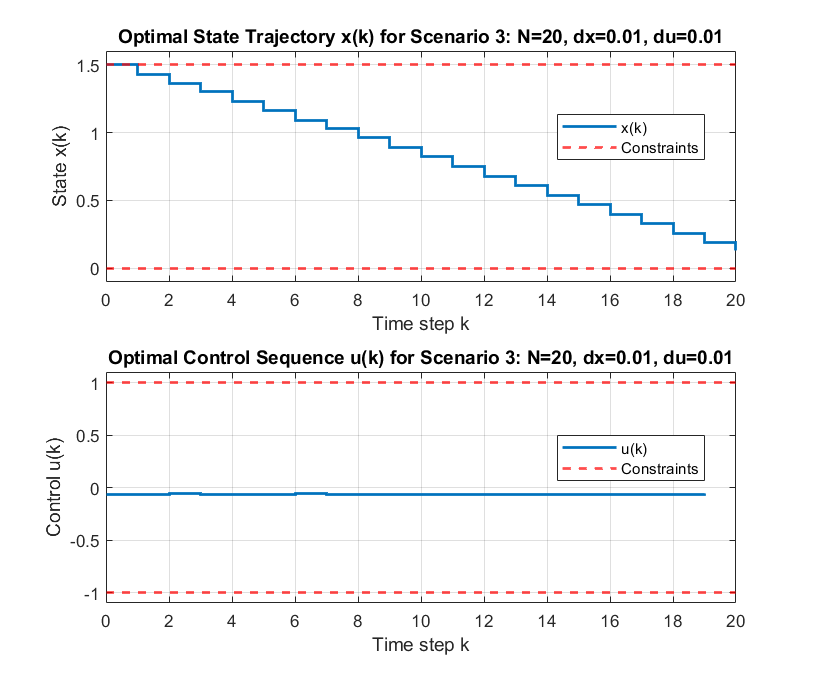
\includegraphics[width=0.48\linewidth]{Q8_3.png}\hfill
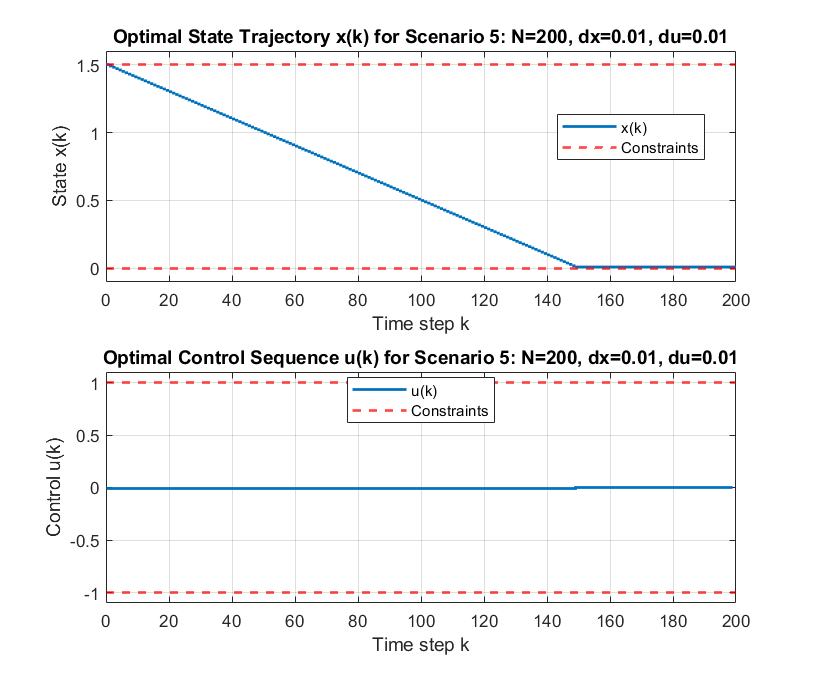
\includegraphics[width=0.48\linewidth]{Q8_5.png}
\end{center}
\textit{Note:} the printed label of scenario 1 in the script says ``dx=0.01'', but the code uses $\Delta x=\Delta u=0.5$, which is the value in the table.
\end{document}
